% !TeX root = ../main.tex
\chapter{TINJAUAN PUSTAKA}

\section{Penelitian Terdahulu}
Penelitian terdahulu yang berkaitan dengan representasi audio, gangguan suara, dan pencarian rekaman burung dirangkum pada Tabel~\ref{tab:penelitian-terdahulu}.

% Ringkasan dan batas klaim: notes/SUMBER_TABEL_2_1_2026-11-05.md.
\begingroup
\setstretch{1.25}
\setlength{\tabcolsep}{3pt}
\setlength{\parskip}{0pt}
\setlength{\LTpre}{18pt}
\setlength{\LTpost}{12pt}
\setlength{\emergencystretch}{2em}
\renewcommand{\arraystretch}{1.0}
% Penyesuaian caption hanya untuk tabel ini: tebal dan rapat ke garis atas.
\makeatletter
\def\LT@makecaption#1#2#3{%
  \LT@mcol\LT@cols c{\hbox to\z@{\hss\parbox[t]\LTcapwidth{%
    \reset@font\bfseries
    \sbox\@tempboxa{#1{#2: }#3}%
    \ifdim\wd\@tempboxa>\hsize
      #1{#2: }#3%
    \else
      \hbox to\hsize{\hfil\box\@tempboxa\hfil}%
    \fi
    \endgraf\vskip6pt}%
  \hss}}}
\makeatother
\newcommand{\kepalaPenelitian}[1]{{\centering\bfseries #1\par}}
\begin{longtable}{@{}>{\centering\arraybackslash}p{0.7cm}>{\raggedright\arraybackslash}p{3.3cm}>{\centering\arraybackslash}p{1.3cm}>{\raggedright\arraybackslash}p{2.4cm}>{\raggedright\arraybackslash}p{2.4cm}>{\raggedright\arraybackslash}p{\dimexpr\linewidth-10.1cm-10\tabcolsep\relax}@{}}
\caption{Penelitian Terdahulu}
\label{tab:penelitian-terdahulu}\\
\hline
\kepalaPenelitian{No.} & \kepalaPenelitian{Judul dan peneliti} & \kepalaPenelitian{Tahun} & \kepalaPenelitian{Data} & \kepalaPenelitian{Metode} & \kepalaPenelitian{Hasil} \\
\hline
\endfirsthead
\multicolumn{6}{c}{\textbf{\tablename~\thetable: Penelitian Terdahulu (lanjutan)}}\\[3pt]
\hline
\kepalaPenelitian{No.} & \kepalaPenelitian{Judul dan peneliti} & \kepalaPenelitian{Tahun} & \kepalaPenelitian{Data} & \kepalaPenelitian{Metode} & \kepalaPenelitian{Hasil} \\
\hline
\endhead
\hline
\endfoot
\hline
\endlastfoot
1 & \textit{Global birdsong embeddings enable superior transfer learning for bioacoustic classification}\newline Ghani, Denton, dan Kahl dkk.~\cite{ghani2023embeddings}
  & 2023
  & Rekaman suara burung, kelelawar, mamalia laut, dan amfibi.
  & Evaluasi vektor fitur (\textit{embedding}) model pralatih, termasuk Perch, menggunakan klasifikator linear.
  & Perch memperoleh kinerja klasifikasi tertinggi pada data yang diuji. \\[6pt]
2 & \textit{On the role of audio frontends in bird species recognition}\newline Ghaffari dan Devos~\cite{ghaffari2024frontends}
  & 2024
  & Rekaman 10 spesies burung Eropa Barat dari Xeno-Canto dan delapan jenis derau dari ESC-50.
  & Perbandingan pengolahan fitur audio untuk pengenalan spesies pada kondisi berderau.
  & Normalisasi dan kompresi meningkatkan ketahanan terhadap derau yang tidak digunakan saat pelatihan. \\[6pt]
% Baris ketiga dilanjutkan pada halaman berikutnya agar ruang halaman terpakai.
3 & \textit{The effect of soundscape composition on}
  & 2023
  & Data 54 spesies di Sonoma County;
  & Klasifikasi suara burung menggunakan CNN
  & Suara manusia berkaitan dengan deteksi keliru, \\
\pagebreak
  & \textit{bird vocalization classification in a citizen science biodiversity monitoring project}\newline Clark, Salas, dan Baligar dkk.~\cite{clark2023soundscape}
  &
  & rekaman lingkungan untuk pengujian mencakup 37 spesies.
  & dan analisis kesalahan berdasarkan suara lingkungan.
  & sedangkan angin berkaitan dengan suara burung yang tidak terdeteksi. \\[6pt]
4 & \textit{BirdNET can be as good as experts for acoustic bird monitoring in a European city}\newline Fairbairn, Burmeister, dan Weisser dkk.~\cite{fairbairn2025birdnet}
  & 2025
  & Rekaman dari satu lokasi di Munich, Jerman; pakar mengidentifikasi 23 spesies.
  & Evaluasi 24 pengaturan BirdNET dan empat tingkat penggabungan waktu berdasarkan hasil pakar.
  & Skor F1 sebesar 0,46--0,84; ambang keyakinan paling berpengaruh terhadap skor tersebut. \\[6pt]
5 & \textit{Klasifikasi Jenis Burung Berdasarkan Suara Kicau Menggunakan Ekstraksi MFCC dan BiLSTM}\newline Janah, Susanto, dan Setiawan~\cite{janah2025mfcc}
  & 2025
  & 750 segmen dari 10 spesies, diperbanyak menjadi 3.750 sampel melalui augmentasi.
  & Ekstraksi MFCC dan klasifikasi menggunakan BiLSTM.
  & Penulis melaporkan akurasi klasifikasi sebesar 98\% pada data uji mereka. \\
\end{longtable}
\endgroup

\section{Bioakustik dan Vokalisasi Burung}

Bioakustik merupakan bidang yang mempelajari suara yang dihasilkan oleh hewan. Dalam pemantauan satwa, rekaman suara dapat digunakan untuk memperoleh informasi tentang keberadaan dan aktivitas hewan tanpa harus mengamati setiap individu secara langsung. Analisis rekaman secara komputasional membantu pengolahan data akustik yang terkumpul, termasuk untuk mengenali suara satwa~\cite{stowell2022bioacoustics}.

Salah satu objek kajian bioakustik adalah vokalisasi burung, yaitu suara yang dihasilkan burung untuk berkomunikasi. Vokalisasi dapat berupa kicauan (\textit{song}) dan panggilan (\textit{call}). Kicauan umumnya berkaitan dengan pembentukan atau pertahanan wilayah dan pemilihan pasangan, sedangkan panggilan dapat digunakan, misalnya, untuk mempertahankan hubungan sosial atau memberikan tanda bahaya. Penggunaan dan bentuk suara tersebut dapat berbeda sesuai spesies dan konteks perilakunya~\cite{lewis2021vocalizations}.

Vokalisasi burung memiliki variasi dalam pola waktu, frekuensi, dan susunan unsur suara, baik antarspesies maupun antarindividu atau populasi dalam spesies yang sama~\cite{lewis2021vocalizations}. Ciri tersebut memberikan informasi yang dapat digunakan dalam analisis rekaman, tetapi suara latar yang muncul bersamaan juga dapat memengaruhi hasil pengenalan~\cite{clark2023soundscape}. Dalam penelitian ini, rekaman vokalisasi digunakan sebagai dasar pencarian berdasarkan kemiripan audio, dengan kesesuaian label spesies sebagai acuan penilaian hasil. Oleh karena itu, pemahaman terhadap variasi vokalisasi membantu menjelaskan pentingnya membandingkan representasi audio ketika kueri mengalami gangguan derau.

\section{Sinyal Audio Digital dan Analisis Waktu--Frekuensi}

Sinyal audio digital merupakan representasi suara sebagai urutan nilai amplitudo yang diambil pada selang waktu tertentu. Banyaknya sampel yang diambil setiap detik disebut laju pencuplikan (\textit{sampling rate}) dan dinyatakan dalam hertz (Hz). Semakin tinggi laju pencuplikan, semakin banyak nilai yang digunakan untuk menggambarkan sinyal dalam satu detik. Dalam pemrosesan bioakustik, urutan nilai tersebut dapat dianalisis secara langsung atau diubah menjadi representasi waktu--frekuensi~\cite{stowell2022bioacoustics}.

Suara burung dapat berubah selama rekaman berlangsung, sehingga informasi frekuensi perlu diamati pada bagian-bagian waktu yang berbeda. Salah satu metode untuk memperoleh informasi tersebut adalah \textit{short-time Fourier transform} (STFT). Metode ini membagi sinyal menjadi bagian pendek atau \textit{frame}, mengalikan setiap bagian dengan fungsi jendela, kemudian menerapkan transformasi Fourier pada setiap bagian. Jendela digeser dengan jarak tertentu (\textit{hop length}) sehingga bagian yang berurutan dapat saling tumpang tindih~\cite{jeon2020stft}. Alur tersebut ditunjukkan pada Gambar~\ref{fig:alur-stft}.

\begin{figure}[htbp]
    \centering
    \jarakSebelumGambar
    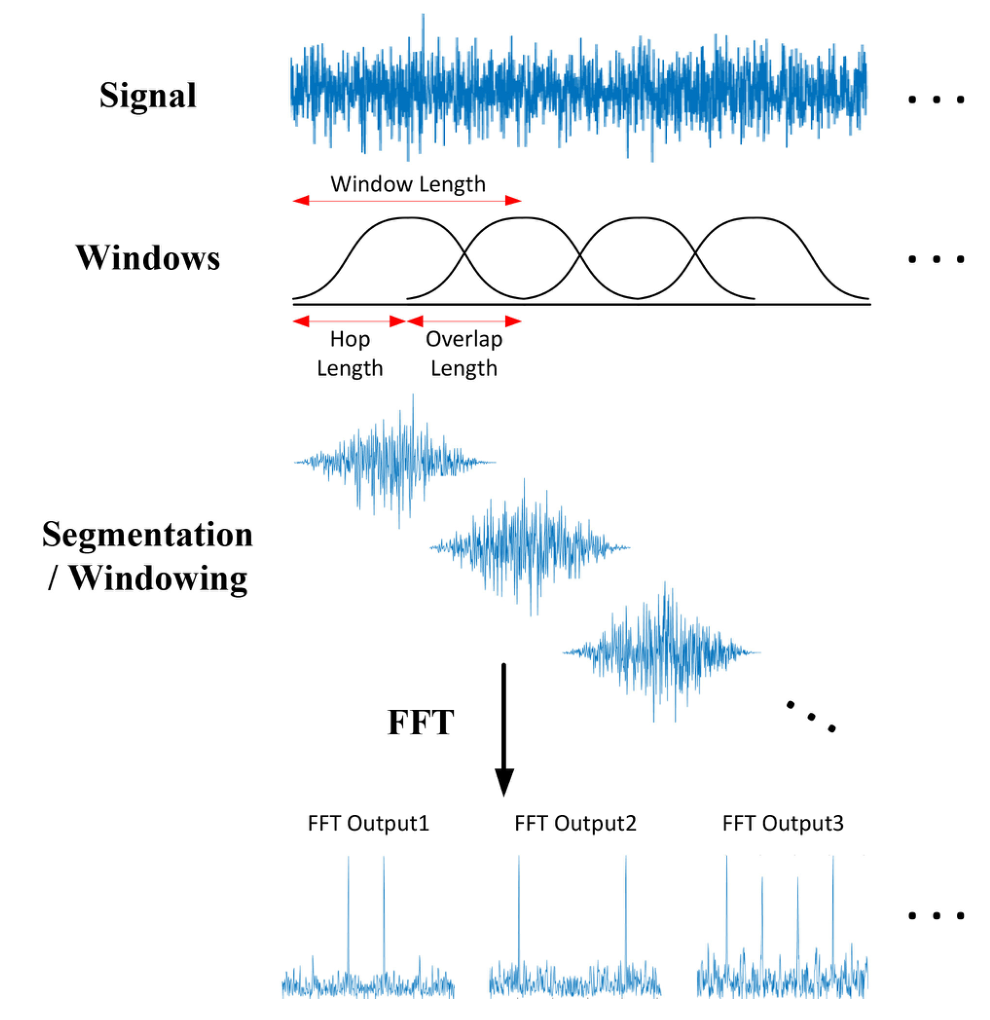
\includegraphics[width=0.65\textwidth]{Gambar/jeon2020_stft.png}
    \caption[Alur analisis sinyal menggunakan STFT]{Alur analisis sinyal menggunakan STFT~\cite{jeon2020stft}}
    \label{fig:alur-stft}
\end{figure}

Menurut Jeon dkk., STFT dapat dinyatakan sebagai berikut~\cite{jeon2020stft}:
\begin{equation}
    X_{\mathrm{STFT}}[k,n] = \sum_{m=0}^{N-1} x[m+nH]w[m]e^{-j2\pi km/N}
    \label{eq:stft}
\end{equation}

\begin{keteranganRumus}
    \hspace{1.5em} \= $X_{\mathrm{STFT}}[k,n]$ \quad \= : \quad \= \kill
    \> $x$ \> : \> sinyal audio digital \\
    \> $w$ \> : \> fungsi jendela \\
    \> $N$ \> : \> panjang jendela dalam sampel \\
    \> $H$ \> : \> jarak pergeseran jendela dalam sampel \\
    \> $n$ \> : \> indeks \textit{frame} \\
    \> $m$ \> : \> indeks sampel dalam jendela \\
    \> $k$ \> : \> indeks frekuensi \\
    \> $j$ \> : \> satuan imajiner \\
    \> $X_{\mathrm{STFT}}[k,n]$ \> : \> hasil transformasi pada frekuensi ke-$k$ dan \textit{frame} ke-$n$
\end{keteranganRumus}

Hasil STFT dapat ditampilkan sebagai spektrogram, yaitu representasi yang menunjukkan kekuatan komponen frekuensi pada setiap bagian waktu. Sumbu mendatar menunjukkan waktu, sumbu tegak menunjukkan frekuensi, sedangkan warna atau tingkat kecerahan menunjukkan besar komponen suara. Representasi ini membantu memperlihatkan pola vokalisasi dan suara latar yang muncul selama rekaman~\cite{stowell2022bioacoustics}. Ghaffari dan Devos menggunakan spektrogram dan spektrogram mel sebagai masukan dalam pengenalan spesies burung, sehingga analisis waktu--frekuensi relevan untuk pengolahan suara burung~\cite{ghaffari2024frontends}.

Dalam penelitian ini, audio disiapkan pada laju pencuplikan 32.000 Hz dengan durasi lima detik. Pada ekstraksi MFCC, analisis menggunakan ukuran transformasi 1.024 sampel dan pergeseran 512 sampel. Parameter tersebut menjelaskan pengolahan pada jalur MFCC; pengolahan internal model pralatih mengikuti kebutuhan masing-masing model.

\section{Prapemrosesan Audio}

Prapemrosesan audio merupakan tahap penyiapan rekaman sebelum analisis atau ekstraksi fitur. Tahap ini diperlukan karena rekaman dapat memiliki format, jumlah kanal, laju pencuplikan, dan durasi yang berbeda. Lu dkk. menyesuaikan rekaman burung menjadi satu kanal dan menyeragamkan laju pencuplikan sebelum analisis~\cite{lu2025dusafnet}. Tahapan yang dipilih bergantung pada tujuan analisis; prapemrosesan tidak selalu berarti menghilangkan derau.

Dalam penelitian ini, rekaman dimuat sebagai audio satu kanal (mono) dan disesuaikan ke laju pencuplikan 32.000 Hz. Rekaman kemudian disiapkan menjadi segmen berdurasi lima detik atau 160.000 sampel. Untuk rekaman yang lebih panjang, beberapa jendela lima detik diperiksa dengan pergeseran 1,25 detik, kemudian jendela dengan nilai \textit{root mean square} (RMS) tertinggi dipilih. Jika rekaman lebih pendek dari lima detik, nilai nol ditambahkan pada bagian akhir hingga panjangnya sesuai.

RMS digunakan untuk mengukur besar amplitudo suatu segmen secara keseluruhan. Lu dkk. menggunakan RMS pada bagian-bagian rekaman burung untuk membantu mendeteksi aktivitas suara~\cite{lu2025dusafnet}. Dengan penyesuaian indeks untuk satu segmen, perhitungan RMS dapat dituliskan sebagai berikut:
\begin{equation}
    \mathrm{RMS}(x)=\sqrt{\frac{1}{N}\sum_{i=0}^{N-1}x[i]^2}
    \label{eq:rms-audio}
\end{equation}

\begin{keteranganRumus}
    \hspace{1.5em} \= $\mathrm{RMS}(x)$ \quad \= : \quad \= \kill
    \> $\mathrm{RMS}(x)$ \> : \> nilai RMS segmen audio \\
    \> $x[i]$ \> : \> amplitudo sampel ke-$i$ \\
    \> $i$ \> : \> indeks sampel \\
    \> $N$ \> : \> jumlah sampel dalam segmen
\end{keteranganRumus}

Nilai RMS yang lebih tinggi menunjukkan amplitudo keseluruhan yang lebih besar, tetapi tidak memastikan bahwa segmen tersebut berisi vokalisasi burung yang paling jelas. Suara latar yang kuat juga dapat menghasilkan RMS tinggi. Oleh karena itu, pemilihan segmen berdasarkan RMS merupakan pendekatan awal dan tidak dianggap sebagai penandaan waktu vokalisasi.

Setelah segmen dipilih, amplitudonya disesuaikan menuju RMS target 0,05. Untuk segmen yang sangat senyap, penyesuaian ini tidak diterapkan; nilai amplitudo kemudian dibatasi pada rentang $-1$ hingga $1$. Pembatasan tersebut dapat menyebabkan RMS akhir berbeda dari target. Penyeragaman ini membantu menyiapkan masukan sebelum ekstraksi representasi, sedangkan derau dalam rekaman tidak dihilangkan melalui normalisasi tersebut.

\section{Derau Aditif dan Signal-to-Noise Ratio (SNR)}

Derau adalah suara yang tidak menjadi sasaran analisis dan dapat muncul bersamaan dengan suara burung. Sumbernya dapat berupa suara angin, hujan, serangga, aktivitas manusia, atau perangkat perekam. Keberadaan suara latar dapat memengaruhi analisis rekaman burung~\cite{clark2023soundscape}. Dalam pencampuran aditif, derau ditambahkan pada rekaman yang menjadi sinyal acuan untuk membentuk kondisi pengujian dengan tingkat gangguan tertentu.

Perbandingan daya sinyal terhadap daya derau dinyatakan sebagai \textit{signal-to-noise ratio} (SNR) dalam desibel (dB). Chen dkk. menjelaskan SNR sebagai perbandingan daya rata-rata sinyal dan derau~\cite{chen2023biotic}. Perbandingan tersebut dalam desibel dapat dinyatakan sebagai berikut:
\begin{equation}
    \mathrm{SNR}=10\log_{10}\left(\frac{P_{s}}{P_{d}}\right)
    \label{eq:snr-daya}
\end{equation}

\begin{keteranganRumus}
    \hspace{1.5em} \= $\mathrm{SNR}$ \quad \= : \quad \= \kill
    \> $\mathrm{SNR}$ \> : \> perbandingan daya sinyal dan derau dalam dB \\
    \> $P_s$ \> : \> daya rata-rata sinyal acuan \\
    \> $P_d$ \> : \> daya rata-rata derau yang ditambahkan
\end{keteranganRumus}

SNR yang lebih besar menunjukkan daya sinyal lebih besar dibandingkan dengan daya derau. Pada SNR 0 dB, daya keduanya sama; pada SNR negatif, daya derau lebih besar daripada daya sinyal. Sebagai contoh, Chen dkk. menunjukkan perubahan tampilan sinyal dan spektrogram ketika SNR berubah dari 35 dB menjadi 0 dB~\cite{chen2023biotic}. Pada Gambar~\ref{fig:contoh-snr}, bagian A dan B menampilkan gelombang, sedangkan C dan D menampilkan spektrogramnya. Skala amplitudo pada bagian A dan B berbeda, sehingga tinggi gelombangnya tidak dibandingkan secara langsung.

\begin{figure}[htbp]
    \centering
    \jarakSebelumGambar
    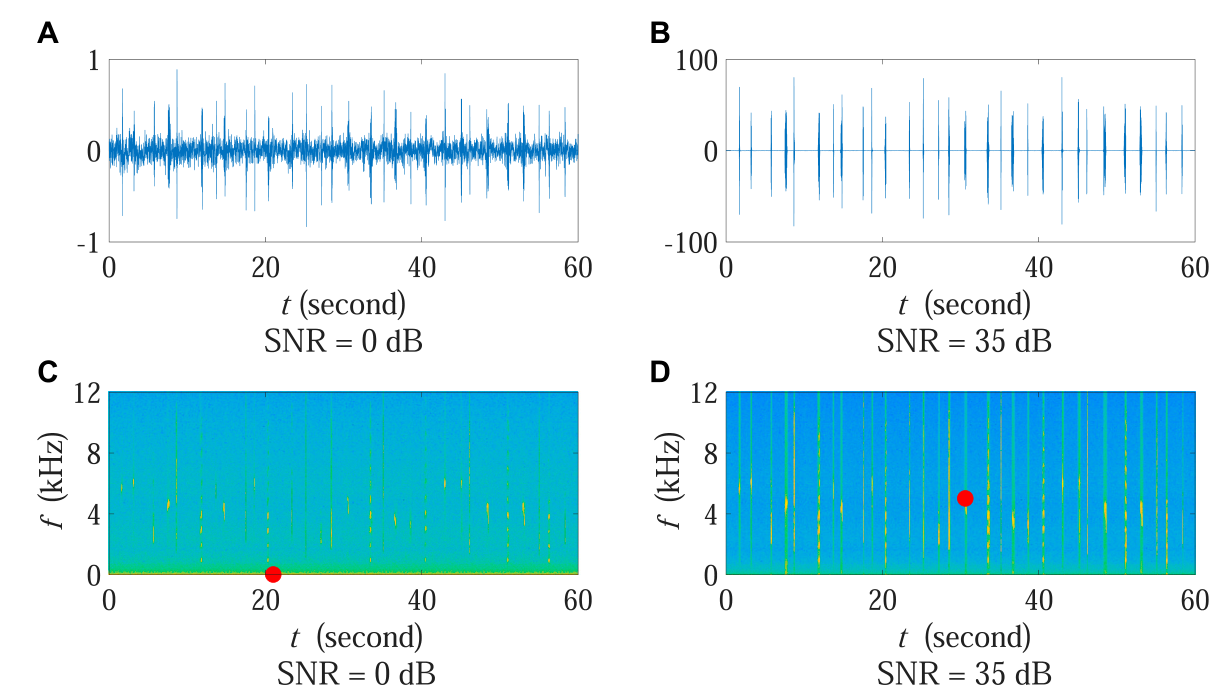
\includegraphics[width=0.93\textwidth]{Gambar/chen2023_snr.png}
    \caption[Contoh sinyal dan spektrogram pada SNR berbeda]{Sinyal dan spektrogram pada SNR 0 dB dan 35 dB~\cite{chen2023biotic}}
    \label{fig:contoh-snr}
\end{figure}

Dalam penelitian ini, rekaman burung tanpa penambahan derau digunakan sebagai sinyal acuan, kemudian dicampur secara aditif dengan rekaman derau lapangan Itera pada SNR $+20$, $+10$, $0$, dan $-5$ dB. Daya derau yang ditambahkan disesuaikan terhadap daya sinyal acuan untuk memperoleh tingkat SNR yang ditentukan. Rekaman acuan tetap dapat mengandung suara latar asalnya, sehingga SNR tersebut menyatakan perbandingan terhadap derau Itera yang ditambahkan, bukan SNR vokalisasi murni. Kondisi tanpa penambahan derau digunakan sebagai pembanding untuk menilai perubahan hasil pencarian.

\section{Mel-Frequency Cepstral Coefficients (MFCC)}

\textit{Mel-frequency cepstral coefficients} (MFCC) merupakan kumpulan koefisien yang merangkum karakteristik spektrum suara pada setiap bagian waktu. Metode ini menggunakan skala mel, yaitu skala frekuensi yang dirancang berdasarkan persepsi pendengaran manusia. Akıncı dan Özbay menjelaskan bahwa koefisien cepstral diperoleh melalui transformasi kosinus terhadap energi berskala mel yang telah dilogaritmakan~\cite{akinci2026mfcc}.

Proses ekstraksi MFCC dimulai dengan pembagian audio menjadi \textit{frame} dan penerapan fungsi jendela. Setiap \textit{frame} dianalisis menggunakan STFT, kemudian energinya dirangkum dalam sejumlah pita frekuensi menggunakan \textit{mel-filter bank}. Setelah operasi logaritma, \textit{discrete cosine transform} (DCT) menghasilkan koefisien MFCC. Peng dkk. menggambarkan tahapan tersebut bersama alur ekstraksi \textit{filter bank} (FBank) pada Gambar~\ref{fig:alur-mfcc}~\cite{peng2025birdfbank}.

\begin{figure}[H]
    \centering
    \jarakSebelumGambar
    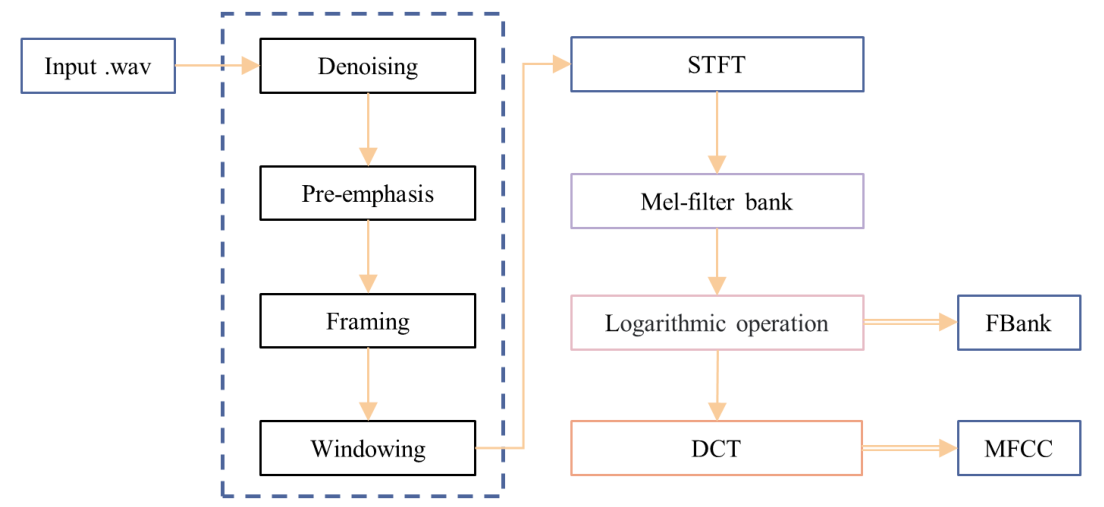
\includegraphics[width=0.95\textwidth]{Gambar/peng2025_mfcc_fbank.png}
    \caption[Contoh tahapan ekstraksi MFCC dan FBank]{Contoh tahapan ekstraksi MFCC dan FBank dari Peng dkk.~\cite{peng2025birdfbank}}
    \label{fig:alur-mfcc}
\end{figure}

Gambar tersebut merupakan alur dalam penelitian Peng dkk. dan juga memuat pengurangan derau (\textit{denoising}) serta \textit{pre-emphasis}. Kedua tahap tersebut tidak diterapkan pada jalur MFCC penelitian ini. Skala mel mengikuti pendekatan pendengaran manusia, sehingga penggunaannya untuk suara burung tetap perlu dievaluasi sesuai data dan tugas yang diteliti~\cite{ghaffari2024frontends}.

Bentuk dasar transformasi MFCC berdasarkan Akıncı dan Özbay dapat ditulis dengan notasi jumlah filter yang dinyatakan secara umum~\cite{akinci2026mfcc}:
\begin{equation}
    c_i = \sum_{k=1}^{K} L_k \cos\left[\frac{\pi i}{K}\left(k-\frac{1}{2}\right)\right]
    \label{eq:mfcc-dct}
\end{equation}

\begin{keteranganRumus}
    \hspace{1.5em} \= $c_i$ \quad \= : \quad \= \kill
    \> $c_i$ \> : \> koefisien MFCC ke-$i$ pada satu \textit{frame} \\
    \> $i$ \> : \> indeks koefisien cepstral \\
    \> $K$ \> : \> jumlah filter pada \textit{mel-filter bank} \\
    \> $k$ \> : \> indeks filter \\
    \> $L_k$ \> : \> logaritma energi keluaran filter ke-$k$
\end{keteranganRumus}

Persamaan tersebut menjelaskan bentuk dasar transformasi; skala dan normalisasi DCT dapat berbeda menurut implementasinya. Dalam penelitian ini, MFCC dihitung menggunakan 20 koefisien untuk setiap \textit{frame}. Nilai setiap koefisien kemudian diringkas sepanjang waktu menggunakan rata-rata dan simpangan baku. Kedua hasil digabungkan menjadi satu vektor berukuran 40 nilai dan dinormalisasi sebelum dibandingkan menggunakan kemiripan kosinus. Dengan cara ini, setiap rekaman memiliki representasi berukuran tetap untuk pencarian.

\section{Representasi Audio Pralatih dan \texorpdfstring{\textit{Frozen Model}}{Frozen Model}}

Representasi audio merupakan cara menyampaikan informasi dalam rekaman sebagai sekumpulan nilai yang dapat diolah oleh sistem. Selain menggunakan fitur seperti MFCC, representasi dapat diperoleh dari model pralatih, yaitu model yang telah melalui proses pelatihan pada kumpulan data sebelumnya. Hasil dari salah satu lapisan model dapat digunakan sebagai vektor fitur atau \textit{embedding}, yang selanjutnya dimanfaatkan untuk tugas analisis lain~\cite{ghani2023embeddings}. Pemanfaatan kembali model pralatih tersebut dikenal sebagai \textit{transfer learning}~\cite{ghani2025generalization}.

Salah satu pendekatan \textit{transfer learning} adalah \textit{frozen model}, yaitu menggunakan model sebagai pengekstrak fitur tanpa memperbarui bobotnya. Pendekatan ini berbeda dari \textit{fine-tuning}, yang memperbarui sebagian atau seluruh bobot melalui pelatihan lanjutan~\cite{ghani2025generalization}. Bobot yang tetap tidak berarti vektor keluarannya selalu sama, karena rekaman yang berbeda dapat menghasilkan \textit{embedding} yang berbeda. Ghani dkk. menggunakan \textit{embedding} dari model berbobot tetap untuk melatih klasifikator bioakustik~\cite{ghani2023embeddings}. Dalam penelitian ini, PANNs CNN14 dan BirdNET digunakan dengan bobot tetap, lalu vektor keluarannya dibandingkan menggunakan kemiripan kosinus untuk mencari rekaman dengan label spesies yang sesuai.

\subsection{PANNs CNN14}

\textit{Pretrained audio neural networks} (PANNs) merupakan kumpulan model jaringan saraf yang dilatih untuk mengenali berbagai jenis suara. Kong dkk. mengembangkan PANNs menggunakan AudioSet, yaitu kumpulan rekaman audio dengan 527 kelas suara. Pelatihan pada beragam kelas tersebut memungkinkan model mempelajari pola audio umum yang dapat dimanfaatkan kembali untuk tugas lain~\cite{kong2020panns}.

Salah satu arsitektur PANNs adalah CNN14, yang menggunakan \textit{convolutional neural network} (CNN) untuk mengolah spektrogram log-mel. Representasi ini menunjukkan distribusi energi suara pada pita frekuensi mel sepanjang waktu. Lapisan konvolusi mempelajari pola pada representasi tersebut, kemudian hasilnya diolah menjadi fitur yang dapat digunakan dalam pengenalan audio~\cite{kong2020panns}.

Dalam penelitian ini, PANNs CNN14 digunakan sebagai pembanding representasi audio umum. Model pralatih dipakai dengan bobot tetap untuk menghasilkan \textit{embedding} berukuran 2.048 nilai dari setiap rekaman. Vektor tersebut dinormalisasi dan digunakan dalam pencarian berdasarkan kemiripan kosinus. Penggunaan ini berfokus pada fitur yang dihasilkan model, sedangkan hasil pengenalan kelas AudioSet bukan keluaran yang dinilai dalam tugas pencarian penelitian ini.

\subsection{BirdNET}

BirdNET adalah model pembelajaran mendalam yang dikembangkan untuk mengenali suara burung. Kahl dkk. menggunakan spektrogram sebagai masukan jaringan saraf untuk mempelajari pola akustik dan menghasilkan prediksi spesies. Penggunaan model ini membantu analisis rekaman dalam pemantauan burung, termasuk rekaman lingkungan yang dapat mengandung beberapa sumber suara~\cite{kahl2021birdnet}.

Model suara burung pralatih juga dapat menghasilkan vektor fitur atau \textit{embedding} untuk tugas bioakustik lain. Ghani dkk. menunjukkan pemanfaatan \textit{embedding} dari model yang dilatih menggunakan suara burung untuk klasifikasi pada beberapa kumpulan data, termasuk rekaman burung dan katak dari Rainforest Connection (RFCX)~\cite{ghani2023embeddings}. Karakteristik model dan data prapelatihannya memberikan dasar untuk membandingkan representasi khusus burung dengan representasi audio umum.

Ketika satu rekaman dibagi menjadi beberapa jendela, vektor \textit{embedding} dari setiap jendela dapat dirata-ratakan untuk memperoleh satu vektor yang mewakili rekaman tersebut. Berdasarkan proses yang dijelaskan oleh Ghani dkk.~\cite{ghani2023embeddings}, perataan tersebut dapat dinyatakan sebagai berikut:
\begingroup\samepage
\begin{equation}
    \bar{\mathbf{e}}=\frac{1}{T}\sum_{t=1}^{T}\mathbf{e}_{t}
    \label{eq:birdnet-mean}
\end{equation}

\begin{keteranganRumus}
    \hspace{1.5em} \= $\bar{\mathbf{e}}$ \quad \= : \quad \= \kill
    \> $\bar{\mathbf{e}}$ \> : \> vektor rata-rata untuk satu rekaman \\
    \> $\mathbf{e}_{t}$ \> : \> vektor \textit{embedding} dari jendela ke-$t$ \\
    \> $T$ \> : \> jumlah jendela dalam satu rekaman \\
    \> $t$ \> : \> indeks jendela
\end{keteranganRumus}
\endgroup

Dalam penelitian ini, BirdNET versi 2.4 digunakan dengan bobot tetap sebagai pengekstrak \textit{embedding}. Audio yang telah disiapkan pada 32.000 Hz disesuaikan ke 48.000 Hz, kemudian diproses dalam jendela tiga detik dengan pergeseran satu detik. Vektor dari setiap jendela dirata-ratakan menjadi satu \textit{embedding} berukuran 1.024 nilai per rekaman dan dinormalisasi sebelum digunakan dalam pencarian.

\section{Audio Similarity Retrieval dan Kemiripan Kosinus}

\textit{Audio similarity retrieval} adalah proses mencari rekaman dalam suatu koleksi berdasarkan kemiripannya dengan rekaman contoh. Rekaman contoh disebut kueri, sedangkan kumpulan rekaman yang ditelusuri disebut koleksi referensi atau \textit{gallery}. Kueri dan setiap rekaman referensi diubah menjadi vektor menggunakan representasi yang sama, lalu dibandingkan untuk memperoleh daftar hasil terurut. Allen-Ankins dkk. menerapkan pencarian suara menggunakan \textit{embedding} BirdNET dengan mengukur kedekatan antara contoh suara dan rekaman dalam koleksi~\cite{allenankins2025retrieval}.

Salah satu cara membandingkan dua vektor adalah kemiripan kosinus (\textit{cosine similarity}), yaitu ukuran yang menunjukkan kesamaan arah kedua vektor. Perhitungannya menggunakan hasil perkalian titik yang dibagi dengan panjang masing-masing vektor. Dengan penyesuaian notasi untuk kueri dan rekaman referensi, rumus tersebut dapat dituliskan sebagai berikut~\cite{milewski2023cosine}:
\begingroup\samepage
\begin{equation}
    \mathrm{sim}(\mathbf{q},\mathbf{g})=
    \frac{\sum_{i=1}^{d}q_i g_i}
    {\sqrt{\sum_{i=1}^{d}q_i^2}\sqrt{\sum_{i=1}^{d}g_i^2}}
    \label{eq:cosine-similarity}
\end{equation}

\begin{keteranganRumus}
    \hspace{1.5em} \= $\mathrm{sim}(\mathbf{q},\mathbf{g})$ \quad \= : \quad \= \kill
    \> $\mathrm{sim}(\mathbf{q},\mathbf{g})$ \> : \> nilai kemiripan kosinus \\
    \> $\mathbf{q}$ \> : \> vektor fitur kueri \\
    \> $\mathbf{g}$ \> : \> vektor fitur rekaman referensi \\
    \> $q_i, g_i$ \> : \> nilai komponen ke-$i$ pada masing-masing vektor \\
    \> $d$ \> : \> jumlah komponen pada setiap vektor
\end{keteranganRumus}
\endgroup

Untuk dua vektor yang tidak bernilai nol, kemiripan kosinus berada pada rentang $-1$ hingga $1$. Nilai yang lebih besar menunjukkan arah vektor yang lebih serupa. Misalnya, rekaman dengan skor $0{,}9$ ditempatkan lebih tinggi daripada rekaman dengan skor $0{,}6$. Skor ini menyatakan kemiripan vektor dan bukan probabilitas bahwa kedua rekaman berasal dari spesies yang sama.

Dalam penelitian ini, setiap kueri dibandingkan dengan rekaman pada koleksi referensi, kemudian hasilnya diurutkan dari skor tertinggi. Relevansi hasil dinilai berdasarkan kesesuaian label spesies. Perhitungan dilakukan secara terpisah untuk masing-masing representasi agar vektor kueri dan referensi berasal dari ruang fitur yang sama. Allen-Ankins dkk. menggunakan jarak Euclidean dalam contoh utama mereka, sedangkan penelitian ini menggunakan kemiripan kosinus untuk pengurutan~\cite{allenankins2025retrieval}.

\section{Metrik Evaluasi Audio Similarity Retrieval}

Evaluasi pencarian menilai kesesuaian dan urutan rekaman yang dihasilkan untuk setiap kueri. Suatu hasil disebut relevan apabila label spesiesnya sama dengan label spesies kueri. Dalam evaluasi informasi, metrik yang berbeda dapat memberikan gambaran yang berbeda pula tentang kualitas suatu urutan hasil~\cite{moffat2022metrics}. Pada penelitian ini, \textit{mean average precision} pada sepuluh hasil teratas (mAP@10) digunakan sebagai metrik utama karena memperhatikan relevansi dan posisi hasil dalam urutan. Metrik pendukung meliputi \textit{precision}@10, \textit{recall}@10, \textit{mean reciprocal rank} (MRR), dan ketepatan hasil pertama (Top-1).

\subsection{\texorpdfstring{\textit{Precision}@10}{Precision@10}}

\textit{Precision}@10 menunjukkan proporsi rekaman yang relevan di antara sepuluh hasil teratas. Untuk satu kueri, ukuran tersebut dapat dinyatakan sebagai berikut~\cite{moffat2022metrics}:
\begin{equation}
    P@10(q)=\frac{\sum_{i=1}^{10}\mathrm{rel}_{q,i}}{10}
    \label{eq:precision-recall}
\end{equation}

\begin{keteranganRumus}
    \hspace{1.5em} \= $P@10(q)$ \quad \= : \quad \= \kill
    \> $q$ \> : \> kueri yang sedang dievaluasi \\
    \> $P@10(q)$ \> : \> \textit{precision}@10 untuk kueri $q$ \\
    \> $\mathrm{rel}_{q,i}$ \> : \> bernilai 1 jika hasil peringkat ke-$i$ relevan; jika tidak, 0
\end{keteranganRumus}

Sebagai contoh, jika empat dari sepuluh hasil teratas relevan, nilai \textit{precision}@10 adalah $4/10=0{,}4$. Nilai ini belum menunjukkan berapa banyak rekaman relevan lain yang terdapat dalam koleksi referensi.

\subsection{\texorpdfstring{\textit{Recall}@10}{Recall@10}}

\textit{Recall}@10 menunjukkan proporsi seluruh rekaman relevan dalam koleksi referensi yang ditemukan pada sepuluh hasil teratas~\cite{sivarajkumar2024clinical}. Untuk satu kueri, perhitungannya dituliskan sebagai berikut:
\begin{equation}
    R@10(q)=\frac{\sum_{i=1}^{10}\mathrm{rel}_{q,i}}{N_q}
    \label{eq:recall10}
\end{equation}

\begin{keteranganRumus}
    \hspace{1.5em} \= $R@10(q)$ \quad \= : \quad \= \kill
    \> $R@10(q)$ \> : \> \textit{recall}@10 untuk kueri $q$ \\
    \> $\mathrm{rel}_{q,i}$ \> : \> penanda relevansi hasil pada peringkat ke-$i$ \\
    \> $N_q$ \> : \> jumlah rekaman relevan bagi kueri $q$ dalam koleksi
\end{keteranganRumus}

Jika empat hasil teratas relevan dan koleksi memiliki 20 rekaman relevan, \textit{recall}@10 bernilai $4/20=0{,}2$. Karena hanya sepuluh hasil yang dihitung, \textit{recall}@10 tidak dapat mencapai satu jika jumlah rekaman relevan dalam koleksi melebihi sepuluh.

\subsection{\texorpdfstring{\textit{Average Precision}@10}{Average Precision@10}}

\textit{Average precision} (AP) juga memperhatikan peringkat setiap hasil relevan. Nilai \textit{precision} dihitung pada setiap posisi yang berisi hasil relevan, kemudian dijumlahkan. Berdasarkan konsep AP yang dijelaskan Moffat~\cite{moffat2022metrics}, penelitian ini membatasi perhitungan hingga sepuluh hasil dan membaginya dengan jumlah terkecil antara banyaknya rekaman relevan dan sepuluh:
\begin{equation}
    AP@10(q)=\frac{\sum_{i=1}^{10}P@i(q)\,\mathrm{rel}_{q,i}}{\min(N_q,10)}
    \label{eq:ap10}
\end{equation}

\begin{keteranganRumus}
    \hspace{1.5em} \= $AP@10(q)$ \quad \= : \quad \= \kill
    \> $AP@10(q)$ \> : \> nilai AP pada sepuluh hasil teratas untuk kueri $q$ \\
    \> $P@i(q)$ \> : \> proporsi hasil relevan hingga peringkat ke-$i$ \\
    \> $\mathrm{rel}_{q,i}$ \> : \> penanda relevansi hasil pada peringkat ke-$i$ \\
    \> $N_q$ \> : \> jumlah rekaman relevan dalam koleksi referensi
\end{keteranganRumus}

Pada perhitungan tersebut, hasil relevan di peringkat awal memberikan kontribusi lebih besar karena nilai \textit{precision} dihitung berdasarkan urutan. Jika tidak ada rekaman relevan dalam koleksi, AP@10 ditetapkan bernilai nol.

\subsection{\texorpdfstring{\textit{Mean Average Precision}@10}{Mean Average Precision@10}}

\textit{Mean average precision} (mAP) merangkum kualitas pencarian untuk sekumpulan kueri dengan merata-ratakan nilai AP setiap kueri~\cite{moffat2022metrics}. Dalam penelitian ini, mAP@10 menjadi metrik utama dan dihitung sebagai berikut:
\begin{equation}
    mAP@10=\frac{1}{|\mathcal{Q}|}\sum_{q\in\mathcal{Q}} AP@10(q)
    \label{eq:map10}
\end{equation}

\begin{keteranganRumus}
    \hspace{1.5em} \= $AP@10(q)$ \quad \= : \quad \= \kill
    \> $mAP@10$ \> : \> rata-rata AP@10 untuk seluruh kueri \\
    \> $AP@10(q)$ \> : \> nilai AP@10 untuk kueri $q$ \\
    \> $\mathcal{Q}$ \> : \> himpunan kueri yang dievaluasi \\
    \> $|\mathcal{Q}|$ \> : \> jumlah kueri dalam himpunan tersebut
\end{keteranganRumus}

Nilai mAP@10 yang lebih tinggi menunjukkan kualitas urutan yang lebih baik secara rata-rata, tetapi bukan persentase ketepatan spesies pada hasil pertama.

\subsection{\texorpdfstring{\textit{Mean Reciprocal Rank}}{Mean Reciprocal Rank}}

MRR menilai seberapa awal hasil relevan pertama muncul dalam daftar. Untuk setiap kueri, peringkat tersebut diubah menjadi nilai kebalikannya, lalu dirata-ratakan pada seluruh kueri~\cite{moffat2022metrics}:
\par\noindent\begin{minipage}{\linewidth}\vspace*{12pt}
\begin{equation}
    MRR=\frac{1}{|\mathcal{Q}|}\sum_{q\in\mathcal{Q}}\frac{1}{r_q}
    \label{eq:mrr}
\end{equation}

\begin{keteranganRumus}
    \hspace{1.5em} \= $MRR$ \quad \= : \quad \= \kill
    \> $MRR$ \> : \> rata-rata kebalikan peringkat hasil relevan pertama \\
    \> $r_q$ \> : \> peringkat hasil relevan pertama untuk kueri $q$ \\
    \> $\mathcal{Q}$ \> : \> himpunan kueri yang dievaluasi \\
    \> $|\mathcal{Q}|$ \> : \> jumlah kueri dalam himpunan tersebut
\end{keteranganRumus}
\end{minipage}\par\addvspace{6pt}

Dalam penelitian ini, peringkat untuk MRR dicari pada seluruh daftar hasil; jika tidak ada hasil relevan, kontribusi kueri tersebut bernilai nol.

\subsection{Ketepatan Hasil Pertama (Top-1)}

Top-1 mengukur proporsi kueri yang hasil peringkat pertamanya relevan. Untuk setiap kueri, penilaian ini setara dengan \textit{precision} pada $k=1$~\cite{moffat2022metrics}: hasil pertama diberi nilai satu jika label spesiesnya sesuai dan nol jika tidak, kemudian nilainya dirata-ratakan untuk seluruh kueri. Nilai \textit{precision}@10 dan \textit{recall}@10 juga dirata-ratakan atas seluruh kueri. Bersama mAP@10, metrik pendukung tersebut memberikan gambaran tentang kualitas urutan, hasil pertama, dan cakupan rekaman relevan yang ditemukan.

\section{Kalibrasi Ambang dan Penerimaan Kueri}

Pencarian berdasarkan kemiripan selalu menghasilkan urutan kandidat ketika koleksi referensi tidak kosong, termasuk untuk kueri yang tidak berasal dari spesies target. Oleh karena itu, diperlukan aturan penerimaan untuk menentukan apakah hasil teratas memiliki skor yang memenuhi ambang yang ditetapkan. Dalam pengenalan suara burung, Fairbairn dkk. menunjukkan bahwa pengaturan ambang memengaruhi hasil evaluasi BirdNET~\cite{fairbairn2025birdnet}. Ambang pada penelitian tersebut berlaku untuk skor kepercayaan klasifikator, sedangkan ambang dalam penelitian ini diterapkan pada skor kemiripan hasil pencarian.

\subsection{Keputusan Penerimaan Berdasarkan Kemiripan}

Pada suatu ambang, kenaikan atau penurunan nilai batas dapat mengubah jumlah hasil yang diterima maupun ditolak~\cite{fairbairn2025birdnet}. Dalam penelitian ini, skor penerimaan kueri diperoleh dari kemiripan kosinus tertinggi terhadap koleksi referensi. Kueri diterima jika skor tertinggi tersebut sama dengan atau melebihi ambang; selain itu, kueri ditolak. Aturan keputusan dapat dituliskan sebagai berikut:
\par\noindent\begin{minipage}{\linewidth}\vspace*{12pt}
\begin{equation}
    s_{\max}(q)=\max_{g\in\mathcal{G}}\mathrm{sim}(q,g),
    \qquad
    A(q)=\left\{\begin{array}{ll}
        1, & s_{\max}(q)\geq\tau,\\
        0, & s_{\max}(q)<\tau.
    \end{array}\right.
    \label{eq:threshold-decision}
\end{equation}

\begin{keteranganRumus}
    \hspace{1.5em} \= $\mathrm{sim}(q,g)$ \quad \= : \quad \= \kill
    \> $q$ \> : \> kueri yang sedang dievaluasi \\
    \> $g$ \> : \> rekaman dalam koleksi referensi \\
    \> $\mathcal{G}$ \> : \> himpunan rekaman referensi \\
    \> $\mathrm{sim}(q,g)$ \> : \> skor kemiripan kueri dan rekaman referensi \\
    \> $s_{\max}(q)$ \> : \> skor kemiripan tertinggi untuk kueri $q$ \\
    \> $\tau$ \> : \> ambang kemiripan \\
    \> $A(q)$ \> : \> keputusan penerimaan; 1 diterima dan 0 ditolak
\end{keteranganRumus}
\end{minipage}\par\addvspace{6pt}

Keputusan tersebut hanya menyatakan apakah skor tertinggi melewati ambang. Kueri target yang diterima belum tentu memperoleh rekaman dengan label spesies yang benar pada peringkat pertama; kesesuaian tersebut dinilai secara terpisah melalui metrik pencarian.

\subsection{Kalibrasi Ambang Menggunakan Indeks Youden}

Kalibrasi merupakan proses memilih ambang berdasarkan data yang telah diketahui kelompoknya. Salah satu kriteria pemilihan ambang adalah indeks Youden, yang menggabungkan sensitivitas dan spesifisitas pada suatu titik batas~\cite{hassanzad2024youden}. Hassanzad dan Hajian-Tilaki membahas kriteria ini dalam analisis diagnostik; pada penelitian ini, konsepnya digunakan untuk membedakan kueri target dari kontrol di luar target berdasarkan skor kemiripan. Indeks Youden dinyatakan sebagai berikut:
\begin{equation}
    J(\tau)=\mathrm{TPR}(\tau)-\mathrm{FPR}(\tau)
    \label{eq:youden-j}
\end{equation}

\begin{keteranganRumus}
    \hspace{1.5em} \= $\mathrm{FPR}(\tau)$ \quad \= : \quad \= \kill
    \> $J(\tau)$ \> : \> nilai indeks Youden pada ambang $\tau$ \\
    \> $\mathrm{TPR}(\tau)$ \> : \> proporsi kueri target yang diterima \\
    \> $\mathrm{FPR}(\tau)$ \> : \> proporsi kontrol di luar target yang diterima \\
    \> $\tau$ \> : \> ambang yang sedang dinilai
\end{keteranganRumus}

Semakin besar nilai $J$, semakin besar selisih antara proporsi penerimaan kueri target dan proporsi penerimaan kontrol di luar target pada data yang digunakan untuk memilih ambang. Pemilihan berdasarkan indeks ini memberi bobot yang sama pada sensitivitas dan spesifisitas, tetapi tidak menjamin kinerja yang sama ketika karakteristik data pengujian berubah~\cite{hassanzad2024youden}.

Dalam penelitian ini, ambang dipilih untuk setiap representasi menggunakan data kalibrasi terpisah tanpa penambahan derau. Kandidat ambang diperoleh dari kurva \textit{receiver operating characteristic} (ROC), kemudian dipilih berdasarkan nilai $J$ tertinggi di antara kandidat yang memenuhi batas pemilihan. Ambang yang diperoleh dipertahankan ketika diterapkan pada data uji tanpa dan dengan penambahan derau, sehingga perubahan keputusan dapat diamati pada aturan penerimaan yang sama.

\subsection{Evaluasi Penerimaan dan Penolakan Kueri}

Sensitivitas dan spesifisitas mengukur kemampuan suatu aturan membedakan dua kelompok pada ambang tertentu~\cite{hassanzad2024youden}. Dalam penelitian ini, kelompok positif adalah kueri target, sedangkan kelompok negatif adalah kontrol di luar target. Hasil keputusan dikelompokkan sebagai penerimaan kueri target yang benar ($TP$), penolakan kueri target ($FN$), penerimaan keliru kontrol di luar target ($FP$), dan penolakan kontrol tersebut ($TN$). Proporsi penerimaan kedua kelompok dihitung sebagai berikut:
\begin{equation}
    \mathrm{TPR}=\frac{TP}{TP+FN},
    \qquad
    \mathrm{FPR}=\frac{FP}{FP+TN}
    \label{eq:acceptance-rates}
\end{equation}

\begin{keteranganRumus}
    \hspace{1.5em} \= $TP$ dan $FN$ \quad \= : \quad \= \kill
    \> $\mathrm{TPR}$ \> : \> proporsi kueri target yang diterima \\
    \> $\mathrm{FPR}$ \> : \> proporsi kontrol di luar target yang diterima \\
    \> $TP$ dan $FN$ \> : \> jumlah kueri target yang diterima dan yang ditolak \\
    \> $FP$ dan $TN$ \> : \> jumlah kontrol di luar target yang diterima dan ditolak
\end{keteranganRumus}

TPR juga disebut \textit{recall} penerimaan, sedangkan FPR menunjukkan tingkat penerimaan keliru pada kontrol. Kedua nilai perlu dibaca bersama: penurunan FPR dapat terjadi bersamaan dengan penurunan penerimaan kueri target. \textit{Recall} penerimaan ini berbeda dari \textit{recall}@10 pada Subbab 2.9.2 karena yang dinilai adalah keputusan terhadap kueri, bukan proporsi rekaman relevan dalam sepuluh hasil teratas.

\section{Ketahanan Derau dan Kestabilan Representasi}

Ketahanan terhadap derau berkaitan dengan kemampuan suatu sistem mempertahankan kualitas hasil ketika masukan mengalami gangguan. Dalam pengenalan suara burung, Ghaffari dan Devos menguji beberapa pengolahan awal audio pada berbagai gangguan dan tingkat SNR untuk melihat perubahan kinerja pengenalan~\cite{ghaffari2024frontends}. Penelitian ini menggunakan gagasan pengujian pada kondisi berderau untuk menilai kualitas urutan pencarian, sehingga metrik dan tugas yang dinilai berbeda dari klasifikasi pada penelitian tersebut.

\subsection{Ketahanan Pencarian terhadap Derau}

Evaluasi ketahanan dapat dilakukan dengan membandingkan hasil pada masukan acuan dan masukan yang diberi gangguan. Besarnya perubahan perlu dilihat pada tugas yang sama, karena ketahanan yang diamati bergantung pada data, jenis gangguan, dan ukuran kinerja yang digunakan~\cite{ghaffari2024frontends}. Dalam penelitian ini, kualitas pencarian pada kueri tanpa penambahan derau dibandingkan dengan kualitas pada kueri yang dicampur derau lapangan Itera pada beberapa tingkat SNR.

Kueri dan koleksi referensi yang digunakan tetap sama pada setiap perbandingan, sedangkan derau ditambahkan pada kueri. Rekaman acuan masih dapat mengandung suara latar asalnya, sehingga istilah tanpa penambahan derau tidak berarti rekaman tersebut bebas dari semua suara latar. Dengan rancangan ini, perubahan mAP@10 menggambarkan perubahan kualitas pencarian pada campuran yang diuji, bukan bukti bahwa kualitas seluruh kondisi perekaman lapangan akan sama.

\subsection{Perubahan Kualitas dan Retensi}

Selain kualitas pada kondisi berderau, perbandingan terhadap kualitas awal membantu menjelaskan seberapa besar kinerja yang berubah. Moffat menjelaskan bahwa makna suatu ukuran evaluasi perlu dibaca sesuai cara ukuran tersebut dibentuk~\cite{moffat2022metrics}. Untuk tujuan penelitian ini, perubahan absolut dan retensi relatif dihitung dari mAP@10 sebagai berikut:
\begin{equation}
    D_m(s)=C_m-A_m(s),
    \qquad
    \rho_m(s)=\frac{A_m(s)}{C_m}
    \label{eq:noise-retention}
\end{equation}

\begin{keteranganRumus}
    \hspace{1.5em} \= $\rho_m(s)$ \quad \= : \quad \= \kill
    \> $m$ \> : \> representasi audio yang dievaluasi \\
    \> $s$ \> : \> tingkat SNR pada pengujian \\
    \> $C_m$ \> : \> mAP@10 tanpa penambahan derau untuk representasi $m$ \\
    \> $A_m(s)$ \> : \> mAP@10 pada tingkat SNR $s$ \\
    \> $D_m(s)$ \> : \> selisih kualitas acuan dan kualitas pada SNR $s$ \\
    \> $\rho_m(s)$ \> : \> retensi relatif terhadap kualitas acuan
\end{keteranganRumus}

Retensi dihitung jika nilai acuan $C_m$ lebih besar dari nol. Sebagai contoh, jika mAP@10 acuan adalah $0{,}8$ dan nilainya pada kondisi berderau menjadi $0{,}6$, retensinya adalah $0{,}6/0{,}8=0{,}75$ atau 75\%. Nilai retensi dapat melebihi 100\% apabila skor pada kondisi berderau lebih tinggi daripada skor acuannya. Karena retensi dipengaruhi nilai awal, hasilnya perlu dibaca bersama mAP@10 pada kedua kondisi.

\subsection{Kestabilan pada Profil Derau yang Berbeda}

Jenis dan karakteristik gangguan dapat menghasilkan perubahan kinerja yang berbeda. Ghaffari dan Devos menguji ketahanan pengenalan terhadap beberapa jenis derau~\cite{ghaffari2024frontends}, sedangkan penelitian ini membandingkan campuran derau lapangan dari lima lokasi Itera pada SNR yang sama. Perbandingan ini menilai variasi hasil pada profil yang dikumpulkan, bukan membuktikan pengaruh setiap sumber suara dalam profil tersebut secara terpisah.

Kestabilan antarprofil diringkas melalui ayunan mAP@10, yaitu selisih antara nilai tertinggi dan terendah di seluruh lokasi pada setiap ulangan, kemudian dirata-ratakan. Ayunan relatif diperoleh dengan membagi ayunan absolut terhadap nilai acuan representasi yang sama:
\par\noindent\begin{minipage}{\linewidth}\vspace*{12pt}
\begin{equation}
    S_m^{\mathrm{abs}}(s)=\frac{1}{R}\sum_{r=1}^{R}
    \left[\max_{l}A_m(s,r,l)-\min_{l}A_m(s,r,l)\right],
    \;
    S_m^{\mathrm{rel}}(s)=\frac{S_m^{\mathrm{abs}}(s)}{C_m}
    \label{eq:location-swing}
\end{equation}

\begin{keteranganRumus}
    \hspace{1.5em} \= $A_m(s,r,l)$ \quad \= : \quad \= \kill
    \> $S_m^{\mathrm{abs}}(s)$ \> : \> rata-rata ayunan mAP@10 antarprofil \\
    \> $S_m^{\mathrm{rel}}(s)$ \> : \> ayunan relatif terhadap mAP@10 acuan \\
    \> $A_m(s,r,l)$ \> : \> mAP@10 pada kombinasi $m$, $s$, $r$, dan $l$ \\
    \> $C_m$ \> : \> mAP@10 acuan tanpa penambahan derau \\
    \> $R$ \> : \> jumlah ulangan pemilihan segmen derau \\
    \> $r,l$ \> : \> indeks ulangan dan lokasi derau
\end{keteranganRumus}
\end{minipage}\par\addvspace{6pt}

Ayunan yang lebih kecil menunjukkan rentang hasil yang lebih sempit pada lokasi dan ulangan yang diuji. Ayunan tersebut tidak langsung menunjukkan kualitas pencarian yang lebih tinggi. Oleh karena itu, nilai absolut dan relatif dibaca bersama; ayunan relatif dihitung hanya ketika nilai acuan lebih besar dari nol. Dalam evaluasi penelitian ini, setiap profil lokasi diuji dengan empat ulangan pemilihan segmen derau.

\section{\texorpdfstring{\textit{Paired Evaluation} dan \textit{Bootstrap}}{Paired Evaluation dan Bootstrap}}

Perbandingan hasil pencarian perlu memperhatikan bahwa kualitas suatu metode dapat berbeda antarrekaman kueri. Evaluasi menggunakan ukuran yang dihitung untuk setiap kueri memungkinkan hasil beberapa metode dibandingkan pada data yang sama~\cite{moffat2022metrics}. Selain nilai rata-rata, penelitian ini menggunakan \textit{bootstrap} untuk membantu menilai ketidakpastian perbandingan berdasarkan variasi kueri yang diamati~\cite{rousselet2021bootstrap}.

\subsection{\texorpdfstring{\textit{Paired Evaluation}}{Paired Evaluation}}

Evaluasi berpasangan membandingkan dua hasil yang berasal dari unit pengamatan yang sama~\cite{faggioli2022smare}. Dalam penelitian ini, setiap rekaman kueri diproses menggunakan representasi atau kondisi yang dibandingkan, kemudian nilai AP@10 dari kueri yang sama dipasangkan. Penggunaan unit kueri sejalan dengan evaluasi kualitas pencarian yang memperhitungkan hasil setiap kueri~\cite{moffat2022metrics}. Sebagai contoh, rata-rata selisih AP@10 antara dua representasi pada suatu kondisi dapat dituliskan sebagai berikut:
\begin{equation}
    \bar{d}=\frac{1}{N}\sum_{i=1}^{N}\left(AP_{A,i}@10-AP_{B,i}@10\right)
    \label{eq:paired-difference}
\end{equation}

\begin{keteranganRumus}
    \hspace{1.5em} \= $AP_{A,i}@10$ \quad \= : \quad \= \kill
    \> $\bar{d}$ \> : \> rata-rata selisih AP@10 antara representasi $A$ dan $B$ \\
    \> $N$ \> : \> jumlah kueri yang dibandingkan \\
    \> $i$ \> : \> indeks kueri \\
    \> $AP_{A,i}@10$ \> : \> nilai AP@10 kueri ke-$i$ pada representasi $A$ \\
    \> $AP_{B,i}@10$ \> : \> nilai AP@10 kueri yang sama pada representasi $B$
\end{keteranganRumus}

Dengan urutan pengurangan tersebut, nilai positif menunjukkan rata-rata AP@10 representasi $A$ lebih tinggi daripada $B$ pada kueri yang dibandingkan. Nilai rata-rata selisih belum menunjukkan besarnya variasi perbandingan, sehingga penilaiannya dilengkapi dengan analisis \textit{bootstrap}.

\subsection{\texorpdfstring{\textit{Paired Bootstrap Resampling}}{Paired Bootstrap Resampling}}

\textit{Bootstrap} adalah metode pengambilan sampel ulang dari data yang tersedia untuk mempelajari variasi suatu statistik. Pada setiap pengulangan, sampel dibentuk dengan mengambil kembali pengamatan secara acak dan mengizinkan pengamatan yang sama terpilih lebih dari satu kali~\cite{rousselet2021bootstrap}. Statistik yang diinginkan kemudian dihitung ulang pada setiap sampel, sehingga diperoleh kumpulan nilai yang dapat digunakan untuk menilai ketidakpastiannya.

Pada \textit{paired bootstrap}, pasangan hasil dari kueri yang sama tetap dipertahankan selama pengambilan sampel ulang. Jika suatu kueri terpilih, seluruh nilai yang dibandingkan untuk kueri tersebut ikut terpilih dengan jumlah kemunculan yang sama. Dalam analisis kestabilan profil derau penelitian ini, indeks kueri yang sama digunakan untuk kedua representasi dan seluruh kondisi yang dibandingkan; nilai acuan tanpa penambahan derau juga dihitung ulang pada setiap sampel. Lokasi dan segmen derau yang digunakan tetap mengikuti data eksperimen.

\subsection{Interval Kepercayaan dan Interpretasi}

Kumpulan nilai hasil pengambilan sampel ulang dapat diringkas menggunakan interval kepercayaan. Rousselet dkk. menjelaskan penggunaan persentil distribusi \textit{bootstrap} untuk menyusun interval kepercayaan~\cite{rousselet2021bootstrap}. Pada pendekatan persentil yang digunakan dalam analisis ini, batas interval kepercayaan 95\% diperoleh dari persentil ke-2,5 dan ke-97,5 kumpulan nilai \textit{bootstrap}:
\begin{equation}
    IK_{95\%}=\left[P_{2{,}5}\!\left(\theta^{*}\right),\;
    P_{97{,}5}\!\left(\theta^{*}\right)\right]
    \label{eq:bootstrap-interval}
\end{equation}

\begin{keteranganRumus}
    \hspace{1.5em} \= $P_{2{,}5}$ dan $P_{97{,}5}$ \quad \= : \quad \= \kill
    \> $IK_{95\%}$ \> : \> interval kepercayaan dengan tingkat 95\% \\
    \> $\theta^{*}$ \> : \> kumpulan nilai statistik dari pengulangan \textit{bootstrap} \\
    \> $P_{2{,}5}$ dan $P_{97{,}5}$ \> : \> persentil ke-2,5 dan ke-97,5 dari kumpulan nilai
\end{keteranganRumus}

Untuk selisih antara dua nilai, interval yang memuat nol menunjukkan bahwa arah perbedaan belum dapat dipastikan berdasarkan interval tersebut. Jika seluruh interval berada di atas atau di bawah nol, arahnya mengikuti urutan pengurangan yang digunakan; hal ini tidak dengan sendirinya menjelaskan penyebab perbedaan. Pada analisis sensitivitas kestabilan antarprofil, pengambilan sampel ulang dilakukan 10.000 kali terhadap kueri secara berpasangan. Interval tersebut bersifat eksploratif dan bergantung pada lokasi serta segmen derau yang digunakan, sehingga tidak mengukur ketidakpastian untuk lokasi atau sesi perekaman baru.

\section{Ciri Spektral dan Analisis Kegagalan}

Ciri spektral merangkum karakteristik sinyal berdasarkan sebaran komponen frekuensinya. Ghani dan Hallerberg menggunakan beberapa ciri audio, termasuk \textit{spectral centroid} dan \textit{spectral bandwidth}, untuk mengolah rekaman pada tugas klasifikasi suara burung~\cite{ghani2021bagbirds}. Dalam penelitian ini, kedua ciri tersebut digunakan untuk mendeskripsikan rekaman yang diperiksa dalam analisis kegagalan pencarian.

\subsection{\texorpdfstring{\textit{Spectral Centroid} dan \textit{Spectral Bandwidth}}{Spectral Centroid dan Spectral Bandwidth}}

\textit{Spectral centroid} menggambarkan pusat sebaran frekuensi sebagai rata-rata frekuensi yang dibobot oleh magnitudo spektrum. Nilai ini dihitung untuk setiap \textit{frame} sebagai berikut~\cite{ghani2021bagbirds}:
\begin{equation}
    C_n=\frac{\sum_{k} f_k S_{k,n}}{\sum_{k} S_{k,n}}
    \label{eq:spectral-centroid}
\end{equation}

\begin{keteranganRumus}
    \hspace{1.5em} \= $S_{k,n}$ \quad \= : \quad \= \kill
    \> $C_n$ \> : \> \textit{spectral centroid} pada \textit{frame} ke-$n$ (Hz) \\
    \> $f_k$ \> : \> frekuensi pada indeks ke-$k$ (Hz) \\
    \> $S_{k,n}$ \> : \> magnitudo spektrum pada frekuensi ke-$k$ dan \textit{frame} ke-$n$ \\
    \> $k,n$ \> : \> indeks frekuensi dan indeks \textit{frame}
\end{keteranganRumus}

Perhitungan tersebut berlaku ketika jumlah magnitudo spektrum tidak nol. Sementara itu, \textit{spectral bandwidth} menggambarkan seberapa lebar sebaran frekuensi di sekitar pusat spektrum~\cite{ghani2021bagbirds}. Ciri dihitung per \textit{frame}, kemudian dirata-ratakan sepanjang rekaman untuk memperoleh satu nilai deskriptif. Nilai kedua ciri dapat dipengaruhi oleh suara burung maupun suara lain dalam rekaman, sehingga tidak dapat digunakan sendiri untuk memastikan sumber suara atau penyebab kegagalan.

\subsection{Analisis Kegagalan Pencarian}

Analisis kegagalan menelaah hasil secara lebih rinci untuk memahami bentuk kesalahan yang tidak terlihat dari nilai rata-rata saja~\cite{clark2023soundscape}. Pada penelitian ini, hasil diperiksa berdasarkan kesesuaian spesies pada peringkat pertama dan keputusan penerimaan terhadap ambang. Contohnya adalah kueri dengan hasil pertama yang sesuai tetapi ditolak oleh ambang, serta kueri yang diterima tetapi hasil pertamanya berasal dari spesies lain.

Untuk membantu membaca kedekatan skor terhadap ambang, selisih antara skor kemiripan tertinggi dan ambang dihitung sebagai \textit{margin}. Nilai positif menunjukkan skor telah mencapai atau melewati ambang, sedangkan nilai negatif menunjukkan skor berada di bawahnya. Informasi ini dibaca bersama ciri spektral dan audit pendengaran pada kasus terpilih. Analisis tersebut bersifat deskriptif; ciri spektral dan hasil pendengaran tidak dengan sendirinya membuktikan penyebab kesalahan atau mewakili seluruh rekaman.

